\section{Extracellular conductivity}
\label{sec:Sigma}
\index{Extracellular conductivity}

\begin{itemize}
\item Experimental measurements \citep{Miceli2017}
\item Theoretical explorations \citep{Meffin2012,Tahayori2012,Meffin2014,Tahayori2014}
\end{itemize}

\begin{figure}[!ht]
\begin{center}
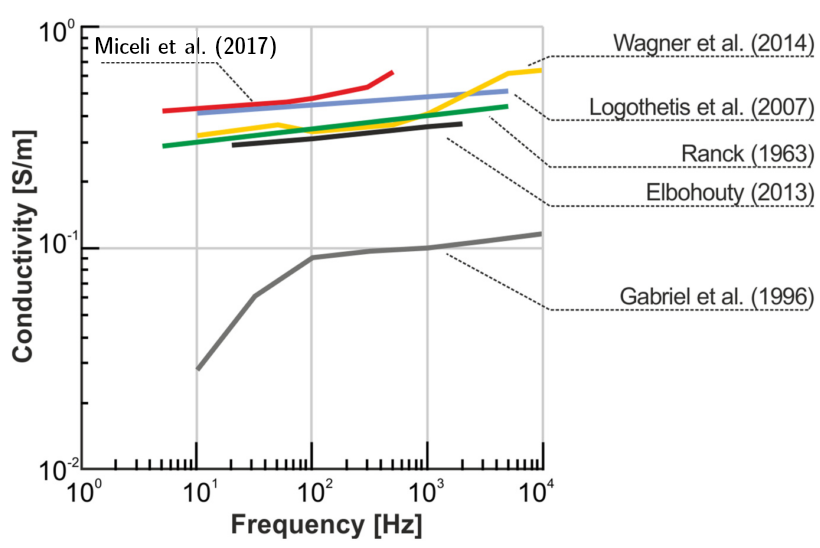
\includegraphics[width=0.6\textwidth]{Figures/Sigma/frequency_dependence.png}
\end{center}
\caption{\textbf{Literature review of reported conductivities in various species and experimental setups.} 
Most studies seem to indicate a very weak frequency dependence of the extracellular conductivity\index{conductivity}, which would have a negligible effect on measured extracellular potentials \citep{Miceli2017}. The very low and strongly frequency dependent values measured by \cite{Gabriel1996} represents an outlier, and although it has received substantial attention, it has to the best of our knowledge not been reproduced by any other study.
For details about the data, see \cite{Miceli2017}, and references therein \citep{Ranck1963, Gabriel1996, Logothetis2007, Elbohouty2013, Wagner2014}
}
\label{Sigma:fig:freq_dep}
\end{figure}


\begin{figure}[!ht]
\begin{center}
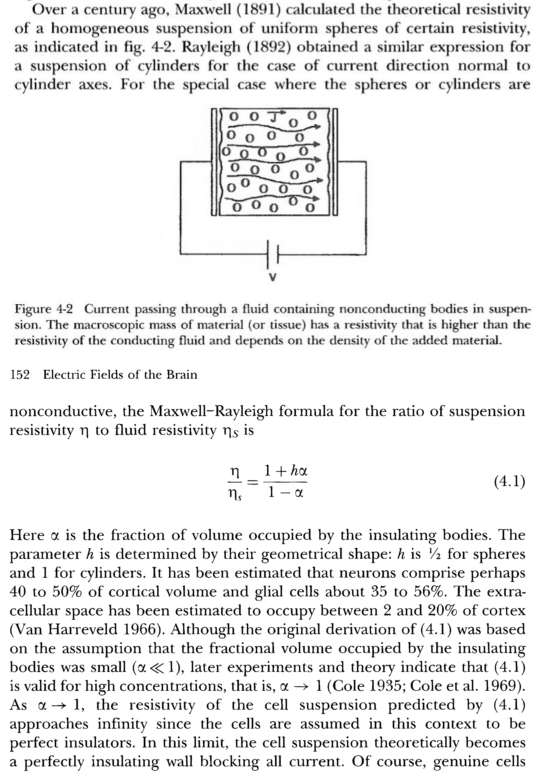
\includegraphics[width=0.6\textwidth]{Figures/Sigma/resistivity_maxwell.png}
\end{center}
\caption{\textbf{From Nunez} \tvnnote{Ta med noe slikt?}}
\label{Sigma:fig:maxwell_resistivity}
\end{figure}

\subsection{Capacitive effects in neuronal tissue}
At high frequencies, extracellular currents could pass through neurons as capacitive currents.
\tvnnote{Utledning tilsvarende Appendix B i Nunez?}


\ghnote{DELKAPITLENE NEDENFOR BLE KLIPPET INN FRA VC-TEORI-KAPITTELET. SATSER PAA AT TORBJORN KAN BRUKE DEM TIL NOE BRA.}

\subsubsection{\orange{Frequency independent conductivity} }
\label{sec:f-independent}
\tvnnote{Her gir det kanskje mest mening å bare oppgi antagelsen om "isotropic, homogeneous and frequency independent conductivity", og henvise til kapittelet om konduktivitet?}
Generally, the response of a medium to an imposed alternating current can depend on the frequency of the current. Then, the conductivity contains a resistive part, which is real and frequency independent, and an imaginary part that account for capacitive and inductive effects that are frequency dependent. In Section \ref{sec:onlyohmic}) we argued that the extracellular displacement current is negligible, which means that the extracellular medium in itself does not exhibit any capacitive effects. This alone does not rule out the possibility that the effective conductivity of the tissue medium includes capacitive effects, as an extracellular current traveling through it could interact with nearby capacitive neural membranes. However, for the relevant frequencies in extracellular recordings, the capacitive and inductive effects appear to be negligible compared to the resistive effects \cite{Logothetis2007, Miceli2017, Ranta2017}. We have therefore based the VC theory presented here on the assumption that the medium is Ohmic or resistive, meaning that we the imaginary and frequency dependent part of the conductivity is zero. We note, however, that it is possible to expand the formalism to include a frequency dependent conductivity \cite{Bedard2004, Tracey2011, Miceli2017}. 


\subsubsection{\orange{Isotropic conductivity} }
A commonly used approximation in VC theory, is that $\sigma$ is isotropic, i.e., the same in all spatial directions. This is mostly an acceptable approximation, and the theory presented in Section \ref{sec:isohomo} relied on this assumption. However, as we showed in Section \ref{sec:anisohomo}, it is possible to expand the formalism to account for an anisotropic conductivities.


\subsubsection{\orange{Homogeneous conductivity} }
Another commonly applied assumption in VC theory, is that the conductivity is the same everywhere, an assumption that we used in Section \ref{sec:isohomo} and Section \ref{sec:anisohomo}, but relaxed in Section \label{sec:nonhomo}. Clearly, this assumption does not hold on the micrometer scale, where neural tissue is highly non-homogeneous \citep{Nicholson1998}. However, microscale inhomogeneities tend to average out on a larger spatial scale (cf. the continuous medium approximation), and a homogeneous conductivity appears to be a reasonable approximation, at least within a given brain region such as cortex \citep{Logothetis2007}. 

When signals are recorded very far from their sources, it is likely that they on their journey have experienced a $\sigma$ that varied on a macroscopic scale. For example, the signals recorded in the EEG have traveled through both brain tissue, bone and skin, which are three different media with different conductivities. When $\sigma$ is non-homogeneos, there is no general analytical formula available (like eqs. \ref{eq:csds} or \ref{eq:anisos}) that link the extracellular potentials to the underlying current sources. Analytical solutions can still be obtained for some simple non-homogeneous cases, such as those presented in Section \ref{sec:nonhomo}. For more general cases, one can in principle always solve eq. \ref{eq:CSD2} for arbitrarily complex geometries with varying conductivities using numerical methods, like the Finite Element Method (FEM) \citep{Logg2012}. For examples of neuroscience applications using this approach, see \cite{Moffitt2005, Frey2009, Joucla2012, Haufe2015, Ness2015, Buccino2019b, Obien2019}. 
